\section{Context and Scope}

Since this system relies on the correct working of external elements, it is important that their interaction is 
corrected displayed.

\subsection{Business Context} \label{business_context}

This graphic is addressed to the following stakeholders: \glsplural{provider}, \glsplural{client} and
Boarding Committee of ``Clean Up the Word (R)''. It should give a black-box view of the interaction the app
and its external components.

\begin{figure}[H]
    \centering
    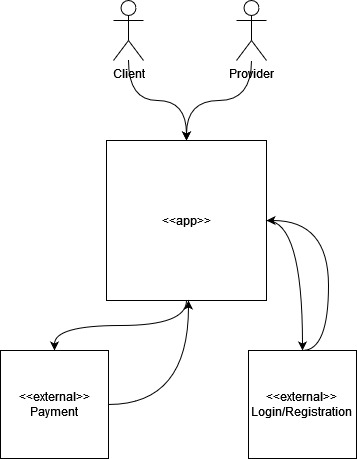
\includegraphics[width=0.5\textwidth]{assets/business_context.jpg}
    \caption{Diagram to describe the business context}
    \label{fig:business_context}
\end{figure}

\begin{table}[H]
    \setstretch{1.0}
    \begin{tabularx}{\textwidth}{lX}
    \toprule
    Artefact & Description   \\
    \midrule
    \gls{client} & Searches for a last time offer from a restaurant, bakery or pastry. \\
    \gls{provider} & Offers a still consumable product that was not sold during normal working time. \\
    Payment & Deals with the payment processing using registered information from another payment platforms. \\
    Login/Registration & Authenticated \glsplural{user} using logins from other platforms.  \\
    \bottomrule
    \end{tabularx}
\end{table}

\subsection{Technical Context}

This following graphic is addressed to our technical team. It provides a white-box view of the previous graphic,
\ref{fig:business_context}.

\begin{figure}[H]
    \centering
    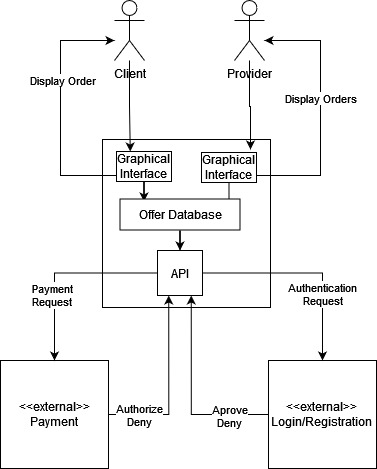
\includegraphics[width=0.5\textwidth]{assets/technical_context.jpg}
    \caption{Technical Context}
    \label{fig:technical_context}
\end{figure}

% \begin{table}[H]
%     \setstretch{1.0}
%     \begin{tabularx}{\textwidth}{lX}
%     \toprule
%     Artefact & Description \\
%     \midrule
%     Graphical Interface & \gls{client} and \gls{provider} have an own interface to interact. \gls{provider} can
%     access view their offer also with a \gls{client}'s perspective. \\
%     Offer Database & \glsplural{client} and \glsplural{provider} can make requests to the database to inquire
%     about its content. \\
%     \gls{api} & For login and payment the authentication and authorization take places on the external service. \\
%     \bottomrule
%     \end{tabularx}
% \end{table}

\begin{table}[H]
    \setstretch{1.0}
    \begin{tabularx}{\textwidth}{lX}
    \toprule
    Artefact & Description \\
    \midrule
    Graphical Interface & \Gls{client} and \gls{provider} have an own interface to interact. \Gls{provider} can
    access view their offer also with a \gls{client}'s perspective. \\
    Offer Database & \Glsplural{client} and \glsplural{provider} can make requests to the database to inquire
    about its content. \\
    \gls{API} & For login and payment the authentication and authorization take places on the external service. \\
    \bottomrule
    \end{tabularx}
\end{table}